% Testes com utilizadores
\chapter{Implementação}
\label{cap4}

%\section{Título de uma seção}
%\subsection{Título de uma subseção}
%\subsubsection{Título de parágrafo de texto normal}

\section{Tecnologias Utilizadas}

Devido à nossa decisão de implementar uma solução que contemplasse tanto hardware e software foi necessário proceder à prototipagem do dispositivo móvel. Vamos em seguida descrever, em primeiro lugar, o hardware utilizado e de seguida o software que escolhemos para criar as interacções.

\FloatBarrier\subsection{Hardware}

Tratando-se do desenvolvimento de um protótipo, que pretende provar o nosso conceito, optamos por utilizar como base de trabalho o SOC \footnote{System on a chip}\cite{ESP8266EX}. Escolhemos este chip, por já estarmos familiarizados com a mesmo e pelo facto de o mesmo já a capacidade de se conectar a ligações WI-FI.

\begin{figure}[!htb]
	\centering
	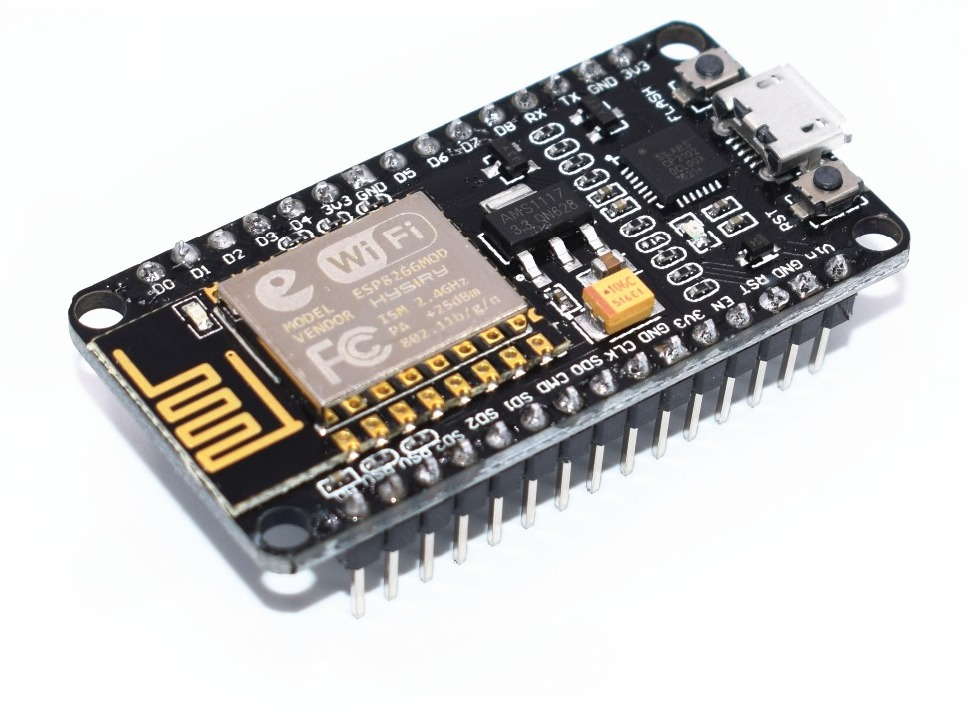
\includegraphics[width=0.4\textwidth]{figuras/ESP8266.jpg}
	\caption{ESP8266}
	\label{fig:ESP8266}
\end{figure}

Para aquisição de dados utilizamos o sensor MPU6050\cite{MPU6050}, que actua como giroscópio e acelerómetro. 

\begin{figure}[!htb]
	\centering
	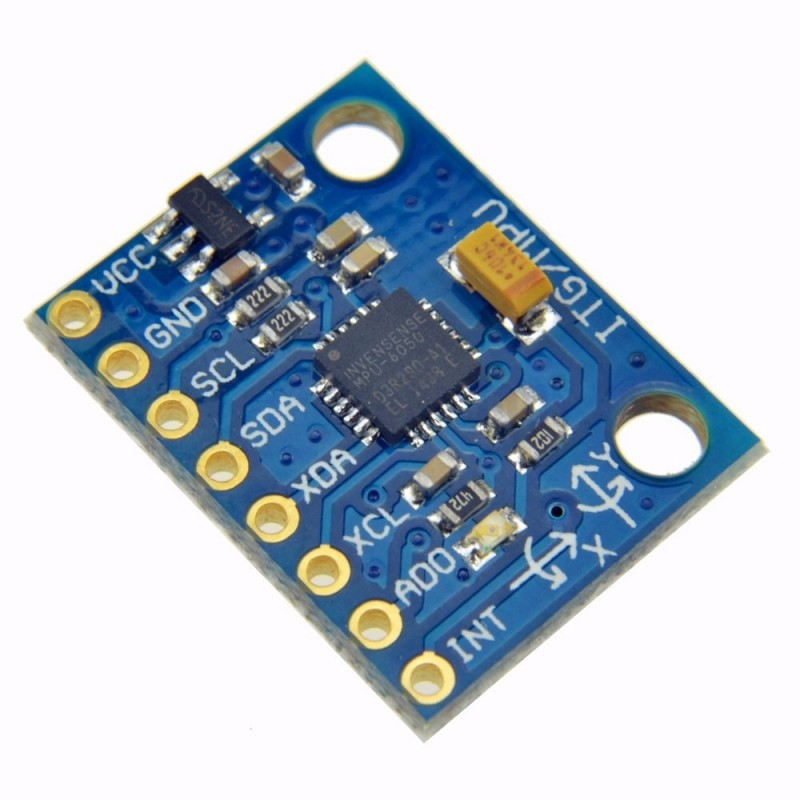
\includegraphics[width=0.4\textwidth]{figuras/MPU6050.jpg}
	\caption{Sensor MPU6050}
	\label{fig:MPU6050}
\end{figure}

Para obter a geolocalização utilizamos o módulo GY-NEO6M v3.0\cite{NEO6}

\begin{figure}[!htb]
	\centering
	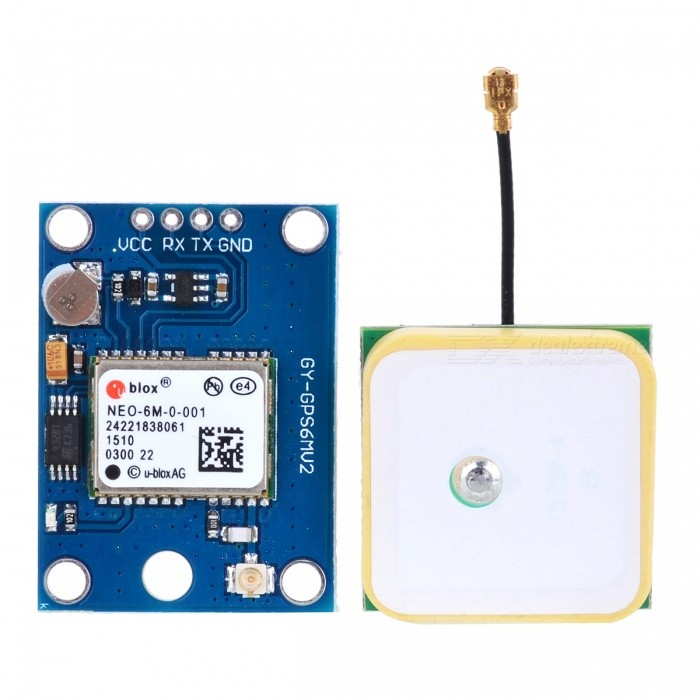
\includegraphics[width=0.4\textwidth]{figuras/NEO6M.jpg}
	\caption{Módulo GPS GY-NEO6M v3.0}
	\label{fig:NEO6M}
\end{figure}

Finalmente utilizamos um botão com capacidade de emitir sinal de radio frequência e uma pequena placa receptora do sinal. Devido ao facto de este ser um material obtido num grande revendedor, e o mesmo não fornecer a ficha técnica do mesmo nem informação adicional não conseguimos apresentar mais detalhes sobre o mesmo.

\begin{figure}[!htb]
	\centering
	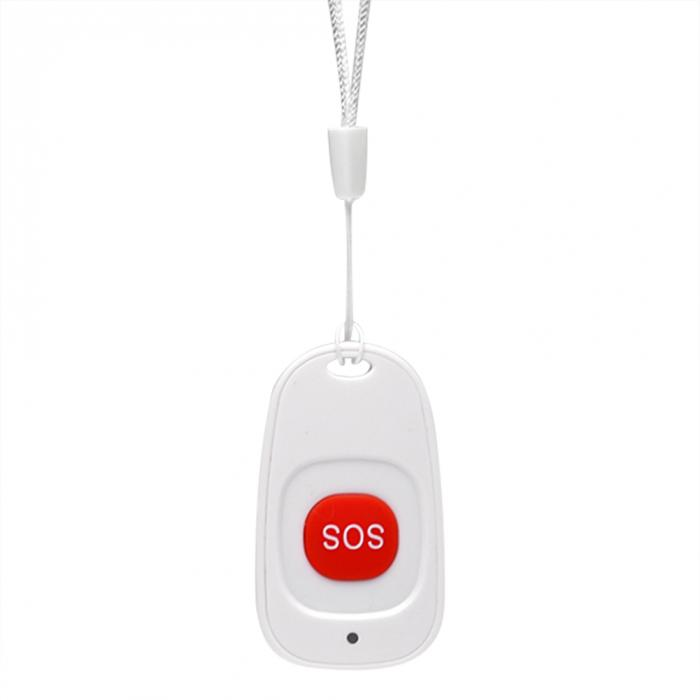
\includegraphics[width=0.6\textwidth]{figuras/SOS_Button.jpg}
	\caption{Botão de SOS}
	\label{fig:SOSbutton}
\end{figure}

\FloatBarrier\subsection{Software}

Em termos de software utilizamos a linguagem de programação Arduino\cite{language} para programar a interacção entre o ESP8266 e o s sensores. Esta linguagem é inspirada em C pelo que fornce fiabilidade, rapidez e flexibilidade.\\
Para a programação do portal que permitia visualizar e interagir com as informações, optamos por utilizar a linguagem PHP\cite{PHP} com a utilização da biblioteca bootstrap\cite{bootstrap} para criar um aspecto mais polido aos documentos HTML e CSS. Utilizamos também a linguagem javascript \cite{javascript} para permitir a interacção entre as páginas. Por opção não utilizamos qualquer tipo de framework, pois consideramos que nesta fase do projecto não havia complexidade suficiente para justificar a utilização da mesma.

\FloatBarrier\subsection{Base de dados}

Um dos requisitos do projecto era a utilização de uma base de dados relacional. Optamos por utilizar o MySQL, pois a mesma integra-se bastante bem com a utilização do phpMyAdmin \cite{phpmyadmin}

\section{Código}

O dispositivo móvel vai estar em loop a obter informação dos botões (remoto e situado no próprio dispositivo) bem como do MPU6050. Estas instruções são as base da detecção e podem ser observadas na listagem \ref{lst:loop_ocorrencia}.

\lstinputlisting[language=C++,caption={Método loop do ESP8266 para detecção das ocorrências.},{label=lst:loop_ocorrencia},firstline=9,lastline=31]{listagens/loop.ino}

No caso de ser detectada uma ocorrência, a geolocalização vais ser pedida ao módulo de GPS, caso este não consiga obter a mesma é enviada a localização do IP. De seguioda é criada uma ligação segura ao servidor, por HTTPS. Estas instrucções podem ser observadas na listagem \ref{lst:loop_ligacao}.

\lstinputlisting[language=C++,caption={Método loop do ESP8266 para ligação ao servidor.},{label=lst:loop_ligacao},firstline=33,lastline=54]{listagens/loop.ino}

De seguida é criada uma linha de texto com as informações relevantes que é enviada para um formulário PHP do lado do servidor, de modo a que possa ser adicionada a nova informação à base de dados. Estas instruções podem ser observadas na listagem \ref{lst:loop_post}.

\lstinputlisting[language=C++,caption={Método loop do ESP8266 para HTTP POST.},{label=lst:loop_post},firstline=63,lastline=103]{listagens/loop.ino}

Do lado do servidor a informação é recebida pelo formulário e separada nas diversas variáveis,que são novamente reformada, desta vez sob a forma de uma query de SQL. É então feita a ligação à base de dados e a query é executada. Estas instruções podem ser observadas na listagem \ref{lst:php_post_data}.

\lstinputlisting[language=PHP,caption={Formulário PHP para insercção de informações na base de dados.},{label=lst:php_post_data},firstline=16,lastline=45]{listagens/post-esp-data.php}

Finalmente é feito uma nova query à base de dados, para determinar quais são os elementos de piquete que se encontram associados à zona da ocorrência e é composto um e-mail que é enviado aos mesmos.  Estas instruções podem ser observadas na listagem \ref{lst:php_email}.

\lstinputlisting[language=PHP,caption={Formulário PHP para envio de e-mail.},{label=lst:php_email},firstline=48,lastline=76]{listagens/post-esp-data.php}

